\chapter{Sparse Grids \textit{\&} Learning}

\section{Sparse Grids}
Sparse grids is a discretization technique that originates from numerical
partial differential equation.
Even though they can be used for diverse problems, we are going to build up
exactly the amount of theory that is useful for our further study.

This chapter starts with a short description of the adaptive sparse grid
technique and then progresses to our application of choice: supervised learning.

\subsection{Basis functions}
\todo{Cite Sparse Grids basics.}
As our first building stone we define the \enquote{mother hat} function
\begin{equation}
  \label{eq:mother-hat}
  \varphi(x) = \max \left( 1 - \vert x \vert , 0 \right).
\end{equation}
\sidetitle{1-Dimensional Basis}
We now define a one-dimensional linear basis function for a level \(l\) and an index \(i\) by
\begin{equation}
  \label{eq:oned-basis}
  \varphi(x)_{l, i} = \varphi(2^l x - i).
\end{equation}
We call the basis function defined by the former equation the linear basis function.
\todo{Check correctness of formula!}
These basis functions assume that the function we want to approximate is zero on
the boundaries.
This is why we use the similarily constructed ``modified linear basis functions'', as defined by Pflüger in~\cite{spatAdaptGrid}:
%https://tex.stackexchange.com/questions/128070/equation-how-to-create-nested-multiple-cases-in-latex-to-align-the-qualifiers
\newlength{\ldiff}
\setlength{\ldiff}{\widthof{$2^l x - i + 1$}-\widthof{$2 - 2^l x$}}
\begin{equation*}
\varphi_j (x) =
  \begin{cases}
    1 & \text {if } l = 1 \land i = 1,\\
    \begin{cases}
      2 - 2^l x & \hspace{\ldiff} \text{if } x \in [0, 2^{1-l}], \\
      0 & \hspace{\ldiff} \text{otherwise},
    \end{cases} & \text{if } l > 1 \land i = 1,\\
    \begin{cases}
      2^l x - i + 1 & \text{if } x \in [1 - 2^{1-l}, 0],\\
      0 & \text{otherwise},
    \end{cases} & \text {if } l > 1 \land i = 2^l - 1,\\
    \varphi(2^l x - i) & \text{otherwise},
  \end{cases}
\end{equation*}
that are identical to the basis functions defined by \cref{eq:oned-basis},
except on the boundaries, where we use extrapolation, for all our experiments.

\todo{Can I use the same notation as bungartz's paper? At least reference it!}
We now define the multi-indices \(\bm{l}\), which denotes the level, and \(\bm{i}\) which indicates the index, i.e.~the position on the grid.
Arithmetical functions act on multi-indices element-wise, we use the relational operator
\begin{equation*}
  \bm{\alpha} \leq \bm{\beta} \iff \forall 1 \leq i \leq \alpha_i \leq \beta_d.
\end{equation*}
The l1- and the maximum-norm are defined as
\begin{equation*}
  \vert \bm{\alpha} \vert_1 = \sum_{1 \leq i \leq d} \alpha_i, \quad \vert \bm{\alpha} \vert_\infty = \max_{1 \leq i \leq d} \alpha_i .
\end{equation*}
We use \(\bm{1}\) and \(\bm{2}\) as a short-hand for \(1, \ldots, 1\) and
\((2, \ldots, 2)\) respectively.

\sidetitle{\(d\)-Dimensional Basis}
We can then construct the d-dimensional basis functions with the following tensor product construction, where we use the one-dimensional basis functions as our building blocks
\begin{equation*}
\varphi_{\bm{l}, \bm{i}} (\bm{x}) = \prod_{k=1}^d \varphi_{l_k, i_k} (x_k).
\end{equation*}

\subsection{Full \textit{\&} Sparse Grids}
Using those basis functions, we can create grids.
The treatment of sparse grids follows~\cite{bungartzSparse}.
Note, that using the index-set
\todo{Fix index set!}
\begin{equation*}
 G_l = \{(l,i) \quad | 1 \leq i_t \leq 2^{l_t} -1, i_t \text{ odd}, 1 \leq t \leq D\}
\end{equation*}
the d-dimensional basis functions span the hierachical subspaces
\begin{equation*}
  W_l = \operatorname{span}\{\phi_{l,i} \in G_l\}.
\end{equation*}
\sidetitle{Full Grid}
Using those subspaces, we can create the set of grid points \(G_n^\infty\) of the full grid for a level \(n\) and its corresponding approximation space \(V_n^\infty\)
\begin{align}
  G_n^\infty &= \bigcup_{\mathclap{\vert {\bm{l}} \vert_\infty \leq n}} G_{\bm{l}}, \\
  V_n^\infty &= \bigoplus_{\mathclap{\vert {\bm{l}} \vert_\infty \leq n}} W_{\bm{l}}.
\end{align}
The number of grid points and thus the degrees of freedom of \(V_n^\infty\) are in \( \BigO (2^{nd})\).
We can represent every function \(f(\bm{x})\) in \(V_n^\infty\) by
\begin{equation}\label{eq:coefficients-h2mix}
  f_{\bm{l}}(\bm{x}) = \sum_{(l,i) \in \bm{G_l}} \alpha_{ki} \varphi_{ki}(\bm{x}),
\end{equation}
as a sum over all grid points that is weighted by the so called hierachical coefficients \(\alpha_{ki}\).

Let \(\Omega = [0, 1]^d\) represent a \(d\)-dimensional interval. 
We now consider functions \(f \from \Omega \to \mathbb{R}\) with bounded mixed second derivatives
\sidetitle{Function Space}
\begin{equation*}
  D^{\bm{\alpha}} f = \frac{\partial^{\vert \bm{\alpha} \vert_1 } f}{\partial x^{\alpha_1}_1 \cdots \partial x^{\alpha_d}_d},
\end{equation*}
where \(\bm{\alpha}\) is a \(d\)-dimensional multi-index.
%\todo{Cite Sobolev space, adjust to otherwise used notation!}
These functions form a Soboloev space \(H_2^\text{mix}(\Omega)\) defined by
\begin{equation*}
  H_2^\text{mix}(\Omega) = \{ f \from \Omega \to \mathbb{R} : D^\alpha \in L_2(\Omega), \vert \alpha \vert_\infty \leq 2, u \rvert_{\alpha \partial = 0}\}
\end{equation*}

\sidetitle{Sparse Grid}
For this function space, sparse grids are a discretization methods that is a
reasonable tradeoff between accuracy and efficiency.
Changing the maximum to the l1-norm we get
\begin{align}
  G_n^1 &= \bigcup_{\vert {\bm{l}} \vert_1 \leq n + d - 1} G_{\bm{l}}, \nonumber \\
  V_n^1 &= \bigoplus_{\vert {\bm{l}} \vert_1 \leq n + d - 1} W_{\bm{l}} \label{eq:sparse-grid-space},
\end{align}
which correspond to the grid point set and the approximation space of sparse
grids respectively.
Df are of order \( \BigO (2^n n^{d-1})\)

\subsection{Adaptivity}
% \begin{figure}[t]
% \centering
% 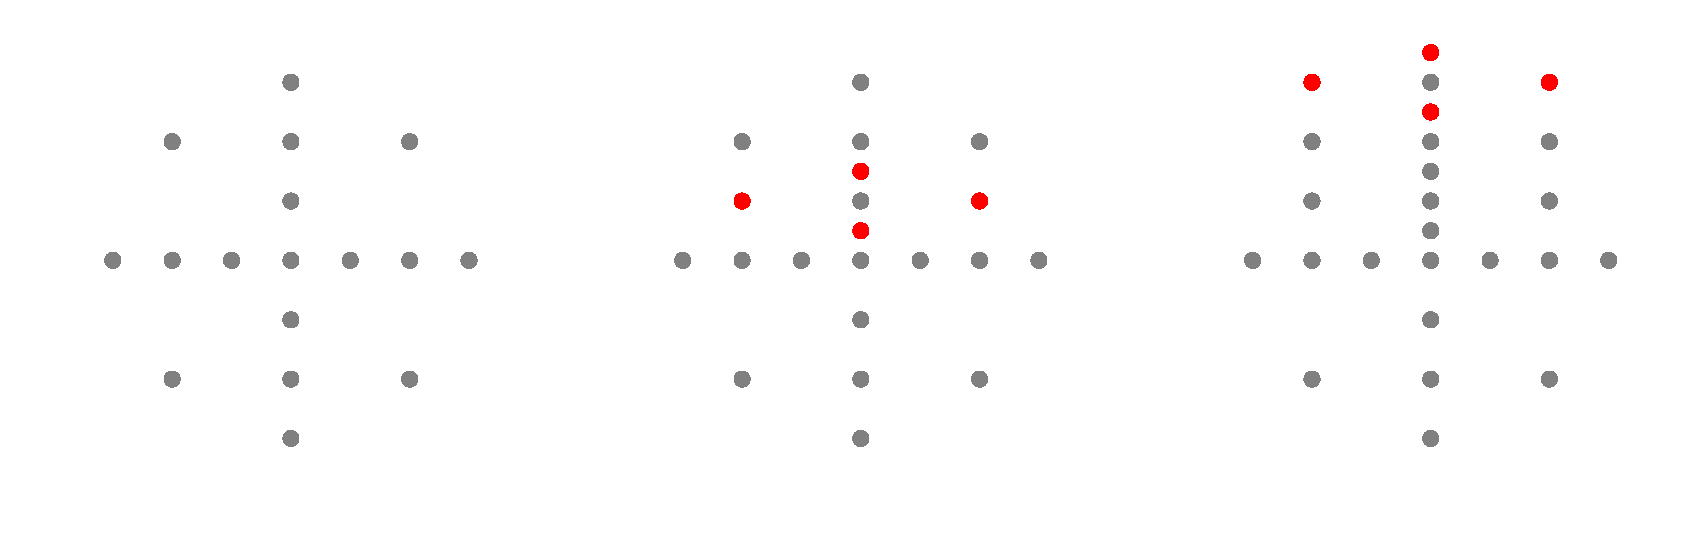
\includegraphics[width=0.7\textwidth]{adaptivity}
% \caption[Adaptivity]{We start with a small 2-dimensional grid with level 3. The first
%   pictures shows the standard grid, the other two show one adaptivity step each.
% The red points are the points that were created by the adaptivity step.}\label{fig:adaptivity}
% \end{figure}
\ldots

\section{Supervised Learning: Regression \textit{\&} Classification}

Consider \ldots \todo{Add concrete example for Regression.}

Let the set \todo{Insert definition for training set.}
\begin{equation*}
T = \left\{ \left(  \bm{x}, y \right) \subset \mathbb{R}^D \times y \right\} 
\end{equation*}
be a set of labeled examples with \(\bm{x}\) as predictors and \(y\) as the
target variable. 
This set is called training set.
We assume that the examples are independent and drawn from the same probability distribution.
\marginline{Our procedure also works, if the examples are dependent. The
  assumption makes the analysis easier.}
Our goal is not interpolation, we do not want to find a function that fits the
examples exactly.
We rather want to find an approximation of our function that
generalizes well, that is a function that allows us to make accurate predictions
for yet unseen, unlabeled data.
In other words we want to learn the structure of the data set.

We differentiate between
\begin{description}
\item[Regression] if we want to predict a continuous \(y\) and
\item[Classification] if we want to predict a discrete value, a class.
\end{description}
In this thesis we will mostly see examples of regression, the last chapter
contains an example for a high-dimensional classification problem.

\section{Inference with Sparse Grids}
We now write:
\begin{equation*}
\boldsymbol{\phi}(\boldsymbol{x}) = \begin{pmatrix}
  \varphi_1(\bm{x}) \\
  \vdots \\
  \varphi_m(\bm{x})
\end{pmatrix}
, \quad
\boldsymbol{\Phi}(\boldsymbol{x}) = \begin{bmatrix}
  \boldsymbol{\phi}(x_1)^\intercal\\
  \vdots \\
  \boldsymbol{\phi}(x_n)^\intercal
\end{bmatrix},
\end{equation*}
which we use to express our regression formula
\begin{equation*}
\hat{y} = \sum_{j = 1}^m \alpha_j \varphi_{j}(\bm{x}) = \boldsymbol{\alpha}^\intercal \bm{\phi} (\bm{x})
\end{equation*}
as a weighted sum of the basis functions.

We can now formulate our goal as an optimisation problem of the form
\begin{equation}\label{eq:optGoal}
\min_{\bm{\alpha}} \left\Vert  \bm{\Phi} \bm{\alpha} - \bm{y}   \right\Vert_2^2  + \lambda \mathcal{S}(\bm{\alpha}), 
\end{equation}
with \(\mathcal{S}(\bm{\alpha})\) as a regularisation operator and \(\lambda\) as a constant.

The procedure explained above also enables us to solve classification problems.
To do this, we perform one-vs-all classification.
This means that we train a learner for each class, and decode the target as 1 if it is a member of our current goal-class and 0 if it belongs to a different class.
To predict the most likely class, we run a prediction for all created estimators and return the class whose learner returned the largest prediction. 

This implies that all methods that improve the performance of the regression procedure are also very likely to lead to better classification results, because we are performing classification via regression.
%%% Local Variables:
%%% mode: latex
%%% TeX-master: "../main"
%%% End: